\documentclass{article}
\usepackage[utf8]{inputenc}
\usepackage{graphicx}
\graphicspath{{.}}

\title{Sprawozdanie z kolokwium PWI}
\author{Anastasiia Dubyna }
\date{November 2020}

\begin{document}

\maketitle

\section{zadanie}

\section{zadanie}
1. Klucze zostały wygenerowane za pomocą ssh-keygen. Dołączam screen potwierdzający to\\ 
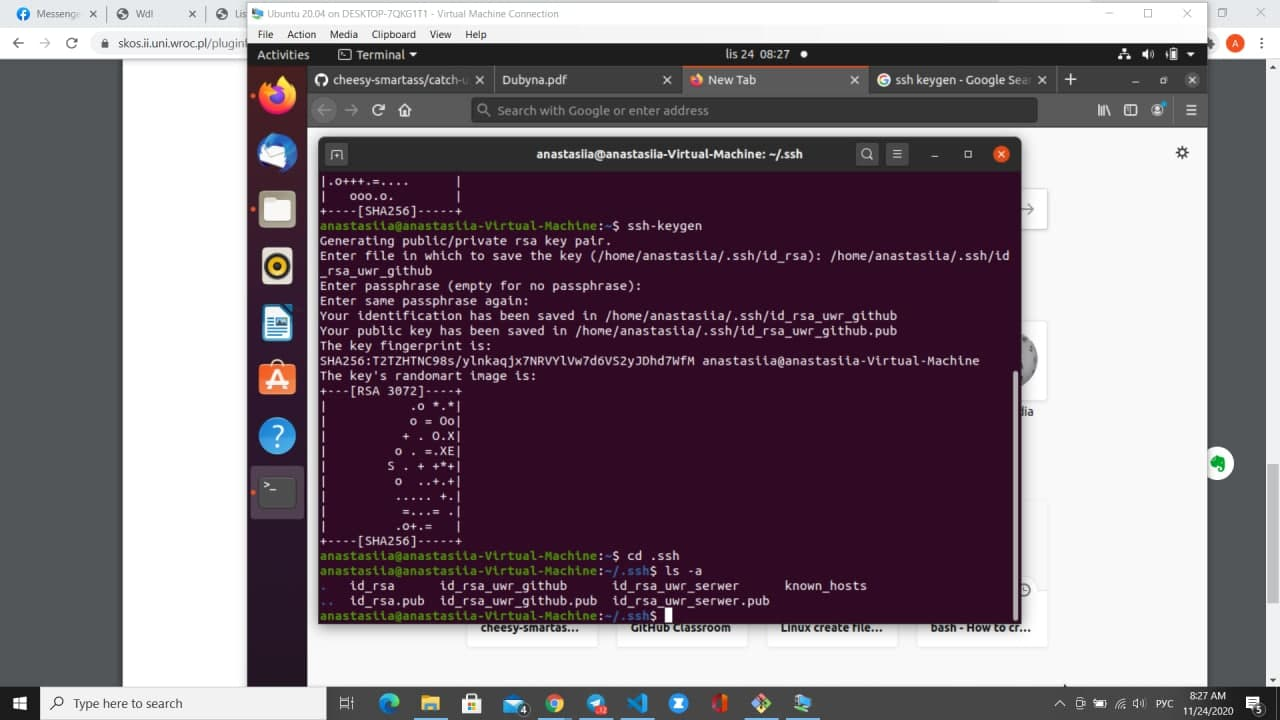
\includegraphics[scale = 0.5]{photo_2020-11-24_08-28-03.jpg}\\
2. Za pomocą ssh-copy-id klucz był przeniesiony na zdalny serwer\\
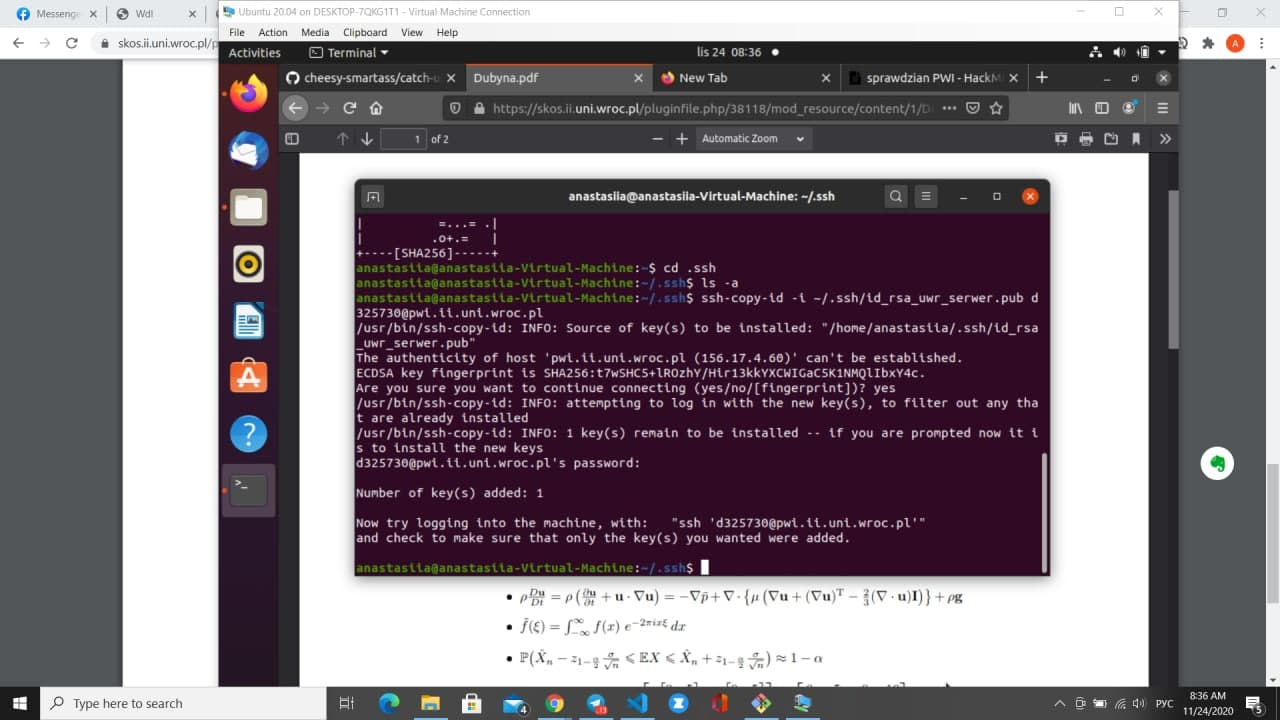
\includegraphics[scale = 0.5]{photo_2020-11-24_09-24-22.jpg}\\
3. Stworzyłam nowe repozytorium na githubie do którego dodałam drugi klucz \\
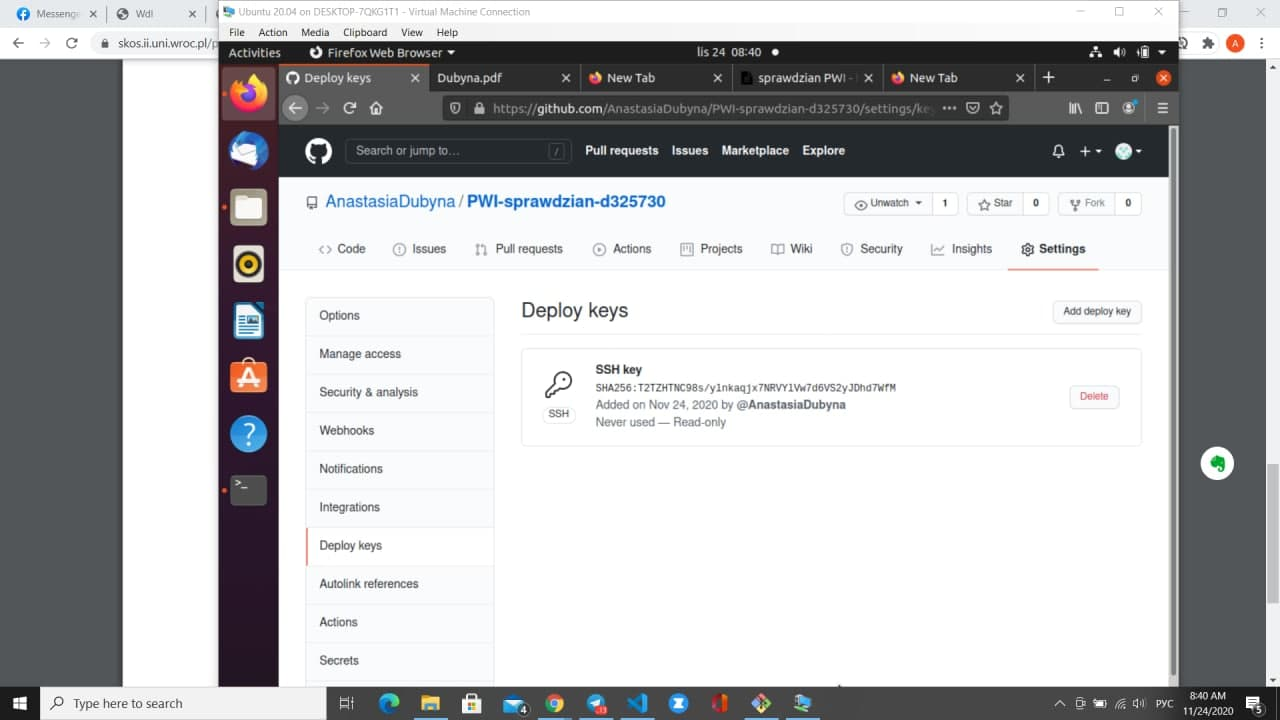
\includegraphics[scale = 0.5]{photo_2020-11-24_09-24-24.jpg}\\
5. Udało się przekierować klucze lokalne za pomocą polecenia ssh -A d325730@pwi.ii.uni.wroc.pl, które pozwala na korzystanie się z authentification agent\\

\section{zadanie}
1. Tak jak w poprzednim zadaniu skorzystałam się z polecenia ssh -A i przeforwardowałąm klucze na serwer
Nie chcemy tworzyć nowej pary kluczy na komputerze zdalnym, bo wtedy ktokolwiek będzie miał dostęp do klucza prywatnego\\
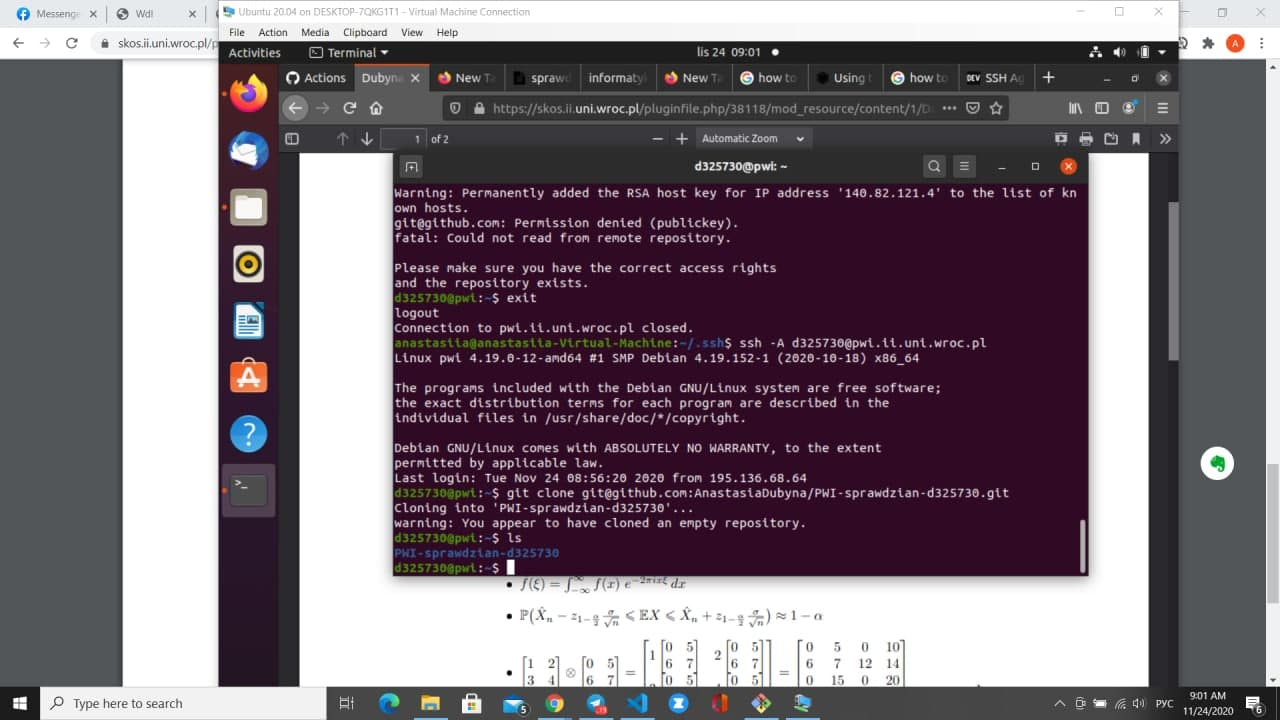
\includegraphics[scale = 0.5]{photo_2020-11-24_09-24-27.jpg}\\

2. Zrobione. wget pozwala ściągnąć pliki z internetu 
tar - wypakowuje archiwum \\
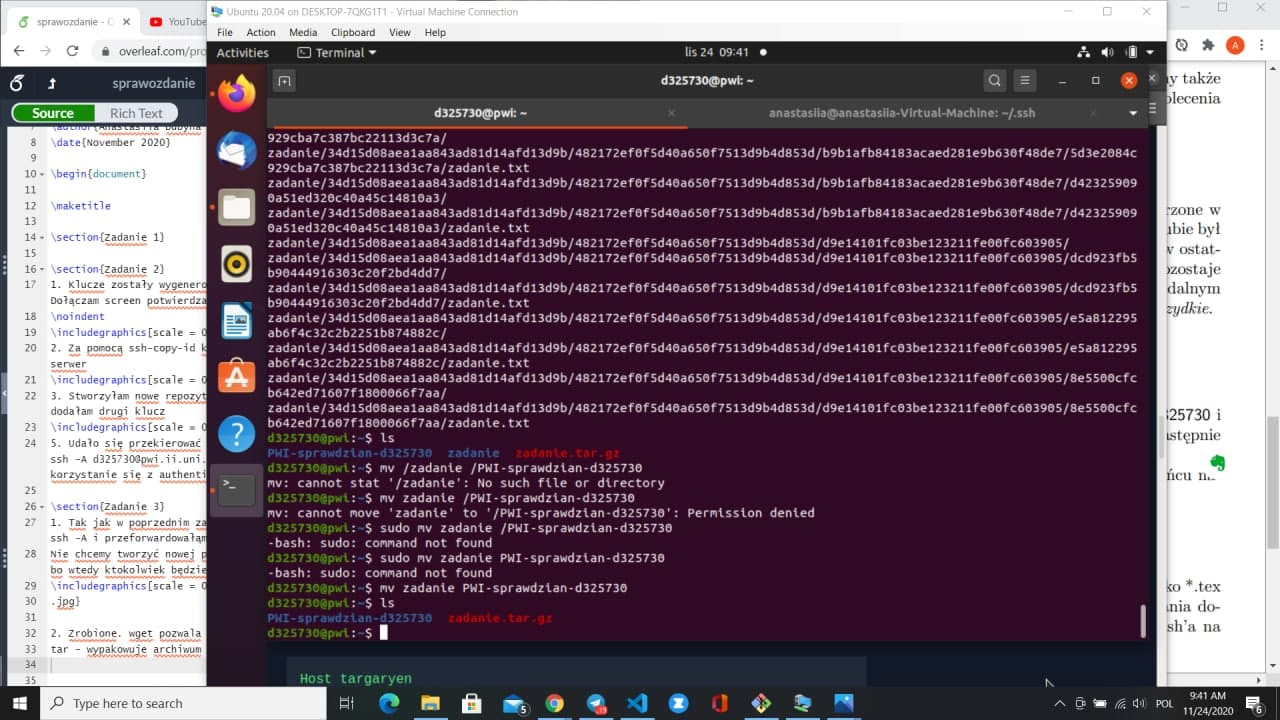
\includegraphics[scale = 0.5]{photo_2020-11-24_09-41-34.jpg}\\

\end{document}
